The interaction of different particles with the nuclei or the
electrons in the gas of the TPC produce different patterns of the 2D
projection of the initial 3D particle trajectory.  These
characteristics, to which we refer generically as ``cluster shapes observables'',
are useful to discriminate different ionizing particles. In particular, they were
used to select a pure sample of nuclear recoil
candidates produced by the interaction of the neutrons originating from the \ambe source and to identify various sources of backgrounds. The main cluster shape observables are described in the following:

\begin{itemize}
  \item \textit{projected length and width:~} a singular value
    decomposition (SVD) on the $x \times y$ matrix of the pixels
    belonging to the supercluster is performed. The eigenvectors found
    can be interpreted as the directions of the two axes of an ellipse
    in 2D. The eigenvalues represent the magnitudes of its semiaxes:
    the major one is defined as \textit{length}, $l$ the minor one
    as \textit{width}, $w$. These are well defined for elliptic
    clusters, or for long and straight tracks. The directions along the
    major and the minor axis are defined as \textit{longitudinal}
    and \textit{transverse} in the following. The longitudinal and
    transverse supercluster profiles, for the cosmic ray track
    candidates shown as an example in Fig.~\ref{fig:super_clusters2}
    (bottom) are shown in Fig.~\ref{fig:profiles}. The longitudinal
    profile shows the typical pattern of energy depositions in
    clusters, while the transverse profile, dominated by the diffusion
    in the gas, shows a Gaussian shape. It has to be noted that the
    cluster sizes represent only the projection of the 3D track in the
    TPC on the 2D $x$--$y$ plane;

    \begin{figure}[ht]
      \begin{center}
        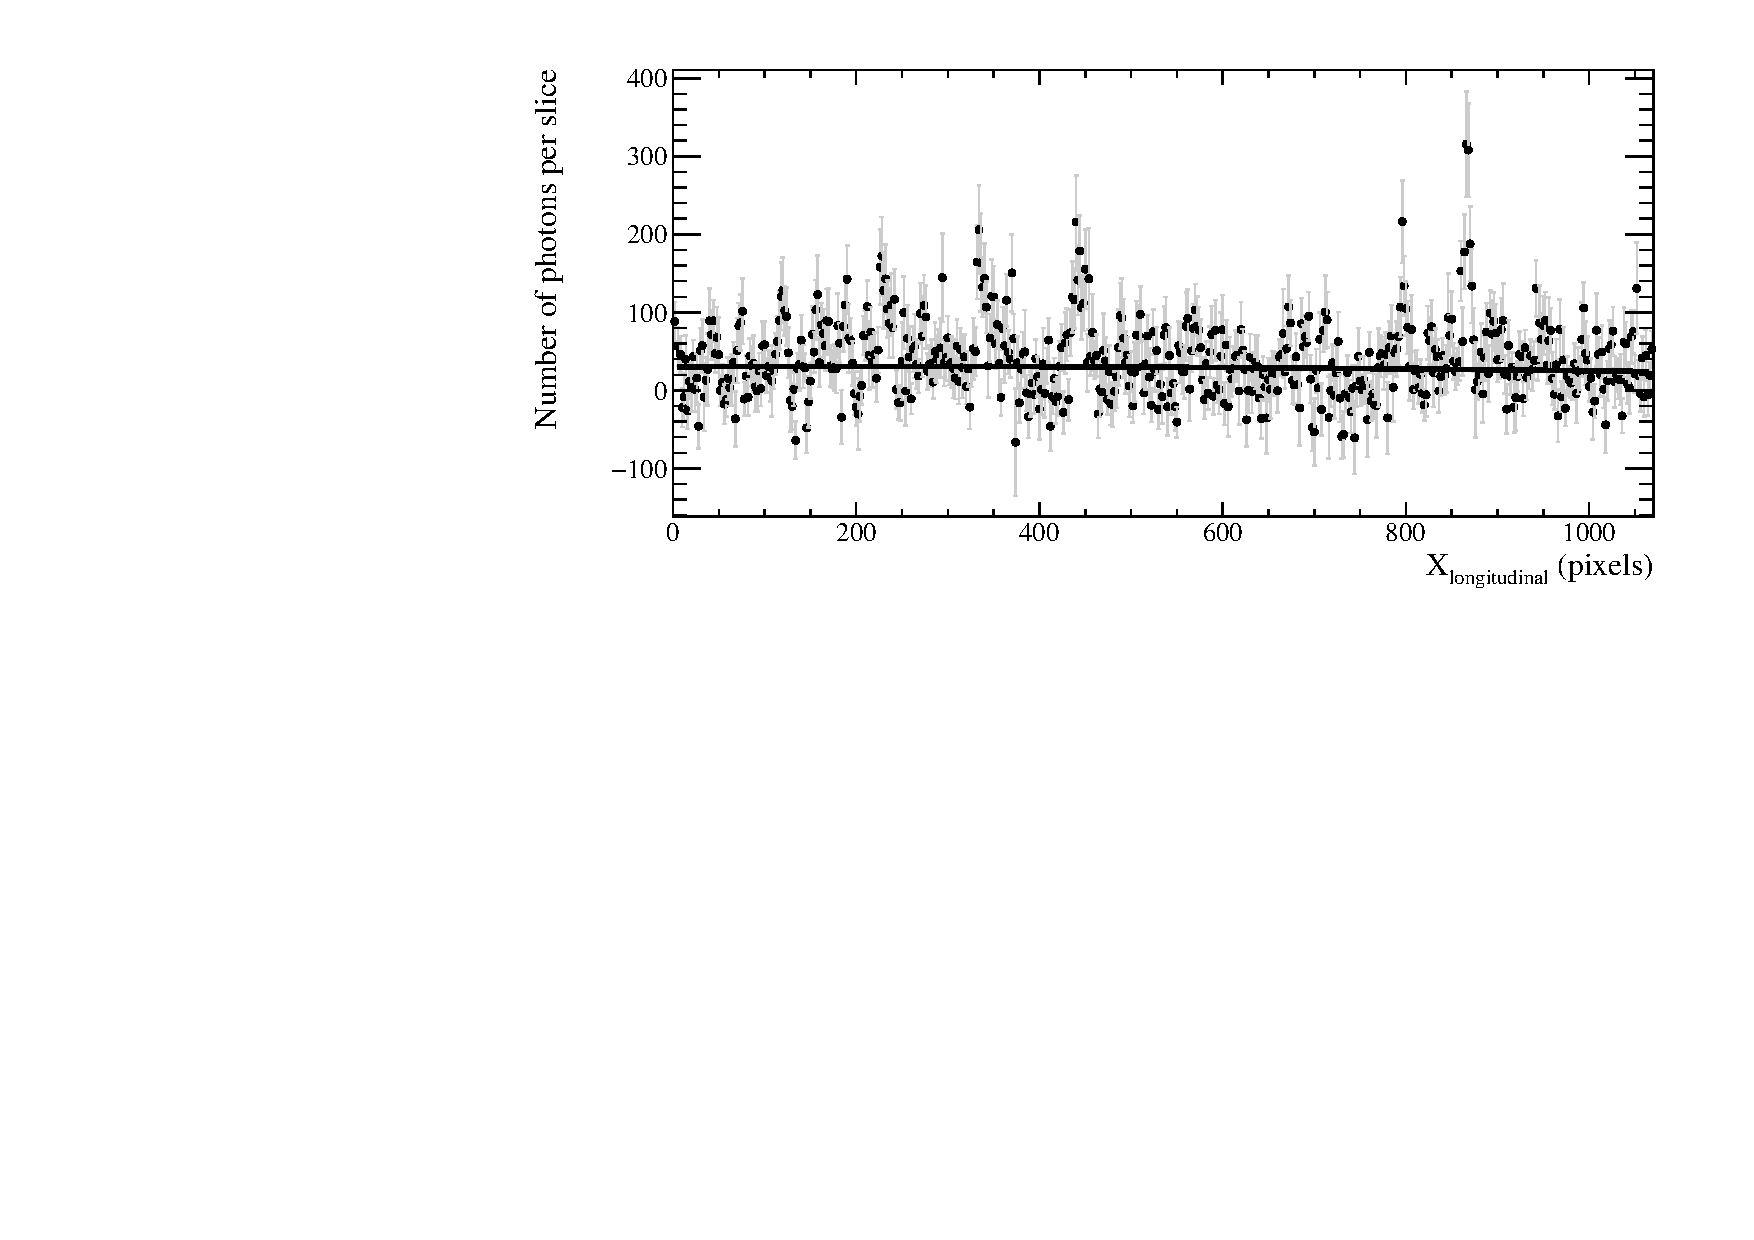
\includegraphics[width=0.45\linewidth]{figures/pic_run02156_ev631_cluster1_longprofile}
        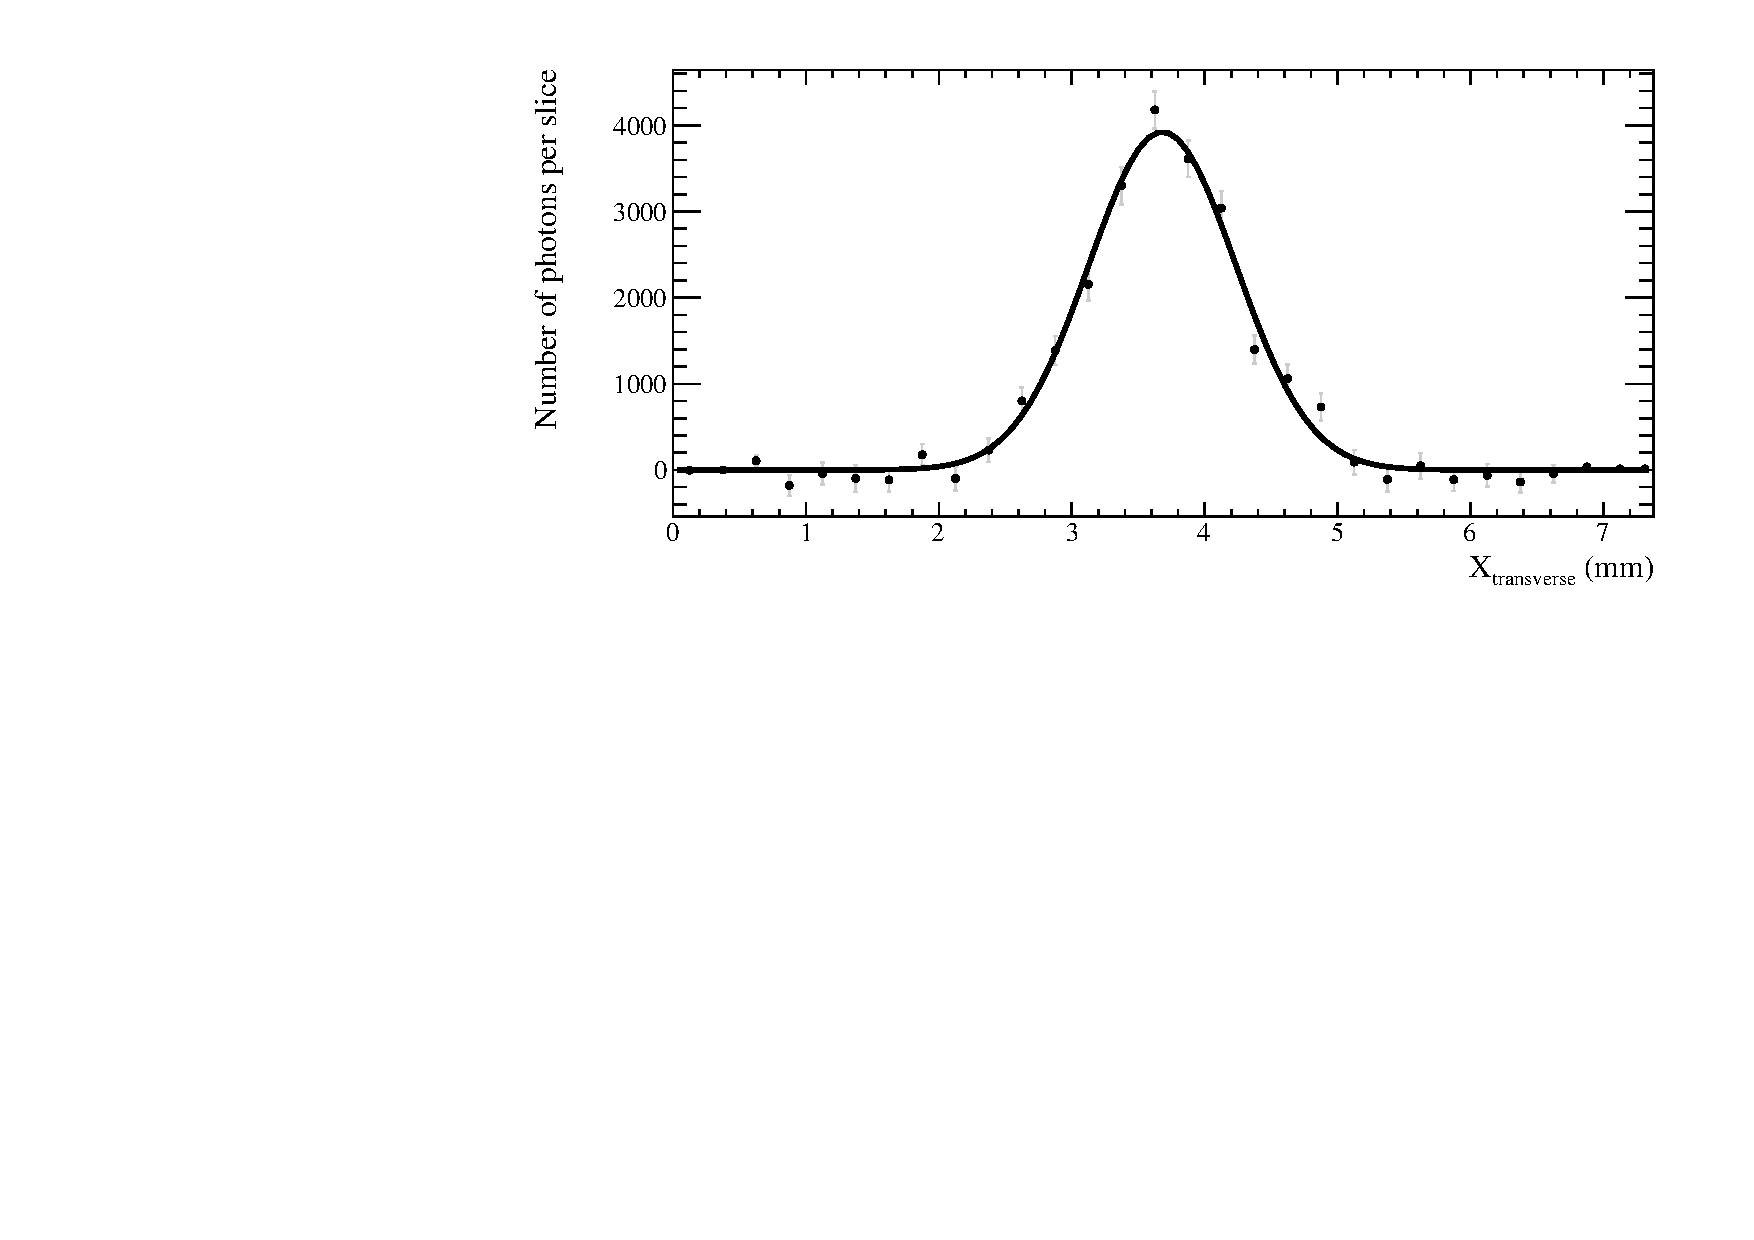
\includegraphics[width=0.45\linewidth]{figures/pic_run02156_ev631_cluster1_latprofile}
        \caption{Supercluster profile in the longitudinal (top) or
          transverse (bottom) direction, for a long and straight
          cosmic ray track candidate shown in  Fig.~\ref{fig:super_clusters2} (bottom). The longitudinal profile shows an
          energy deposition in sub-clusters, while the transverse
          direction shows the typical width of the diffusion in the
          gas. For the longitudinal profile, the line represent the
          average number of photons per slice. For the transverse
          profile, it represents a fit with a Gaussian
          PDF. \label{fig:profiles}}
      \end{center}
    \end{figure}

  \item \textit{projected path length:~} for curly and kinky tracks
    the values returned by the SVD of the supercluster are not an
    accurate estimates of their size. While the width is dominated by
    the diffusion, the length for patterns like the one shown in the
    example of Fig.~\ref{fig:super_clusters1} is ill-defined. In these
    cases, the path length, $l_p$, computed with the skeletonization
    procedure in Fig.~\ref{fig:skeleton} is used;

  \item \textit{Gaussian width:~} the original width of the track in the
    transverse direction is expected to be much lower than the observed width induced by the diffusion in the gas. Thus, as shown in
    Fig.~\ref{fig:profiles} (right), the standard
    deviation, \tsigmag, can estimated by a fit with a Gaussian
    probability density function (PDF);

  \item \textit{slimness:~} the ratio of the width over length,
    $\xi=w/l$, represents the aspect ratio of the cluster. It is very
    useful to discriminate between cosmic rays-induced background
    (long and thin) from low energy nuclear or electron recoils (more
    elliptical or round, as the \fe spots);
    
  \item \textit{integral:~} the total number of photons detected by all the
  pixels gathered in the supercluster, \isclu, as defined in
  Eq.~\ref{eq:integral};

  \item \textit{pixels over threshold:~} the number of pixels in the
  supercluster passing the zero-suppression threshold, $n_p$;

  \item \textit{density:~} the ratio $\delta$ of \isclu, divided by
  $n_p$, as defined in Eq.~\ref{eq:density};

  \item \textit{energy:~} the calibrated energy, expressed
    in \keV. The calibration method simultaneously performs both the
    per-slice correction as a function of the local $\delta$, and the
    absolute energy scale calibration, which corrects the non perfect
    containment of the cluster, using with \fe source.
\end{itemize}

The projected supercluster path length, $l_p$, and Gaussian transverse
size, \tsigmag, are shown in Fig.~\ref{fig:clsize}, for data taken in
different types of runs.  During the data-taking approximately 3000
frames were recorded in absence of any external artificial source ({\it
no-source} sample). In these frames the interaction of
ultra-relativistic cosmic ray particles (mostly muons) are clearly
visible as very long clusters. Internal radioactivity of the \lemon
materials also contribute with several smaller size clusters. About
1500 frames were acquired with the \ambe source, and approximately
$10^4$ calibration images with \fe source. In  Fig.~\ref{fig:clsize}, as well as
in the following ones showing other cluster properties, the
distributions obtained in runs  without artificial radioactive sources are normalized
to the \ambe data total CMOS exposure time. For the data with \fe source,
since the activity of the source is such to produce about 15
clusters/event, the data are scaled by a factor one-tenth with respect to the \ambe
exposure time for clearness. Considerations about the trigger
efficiency scale factor between data with and without an artificial  source are
detailed later. The distributions in this section aim to show
the different cluster shape observables  among the  different kinds of
events.

\begin{figure}[ht]
  \begin{center}
  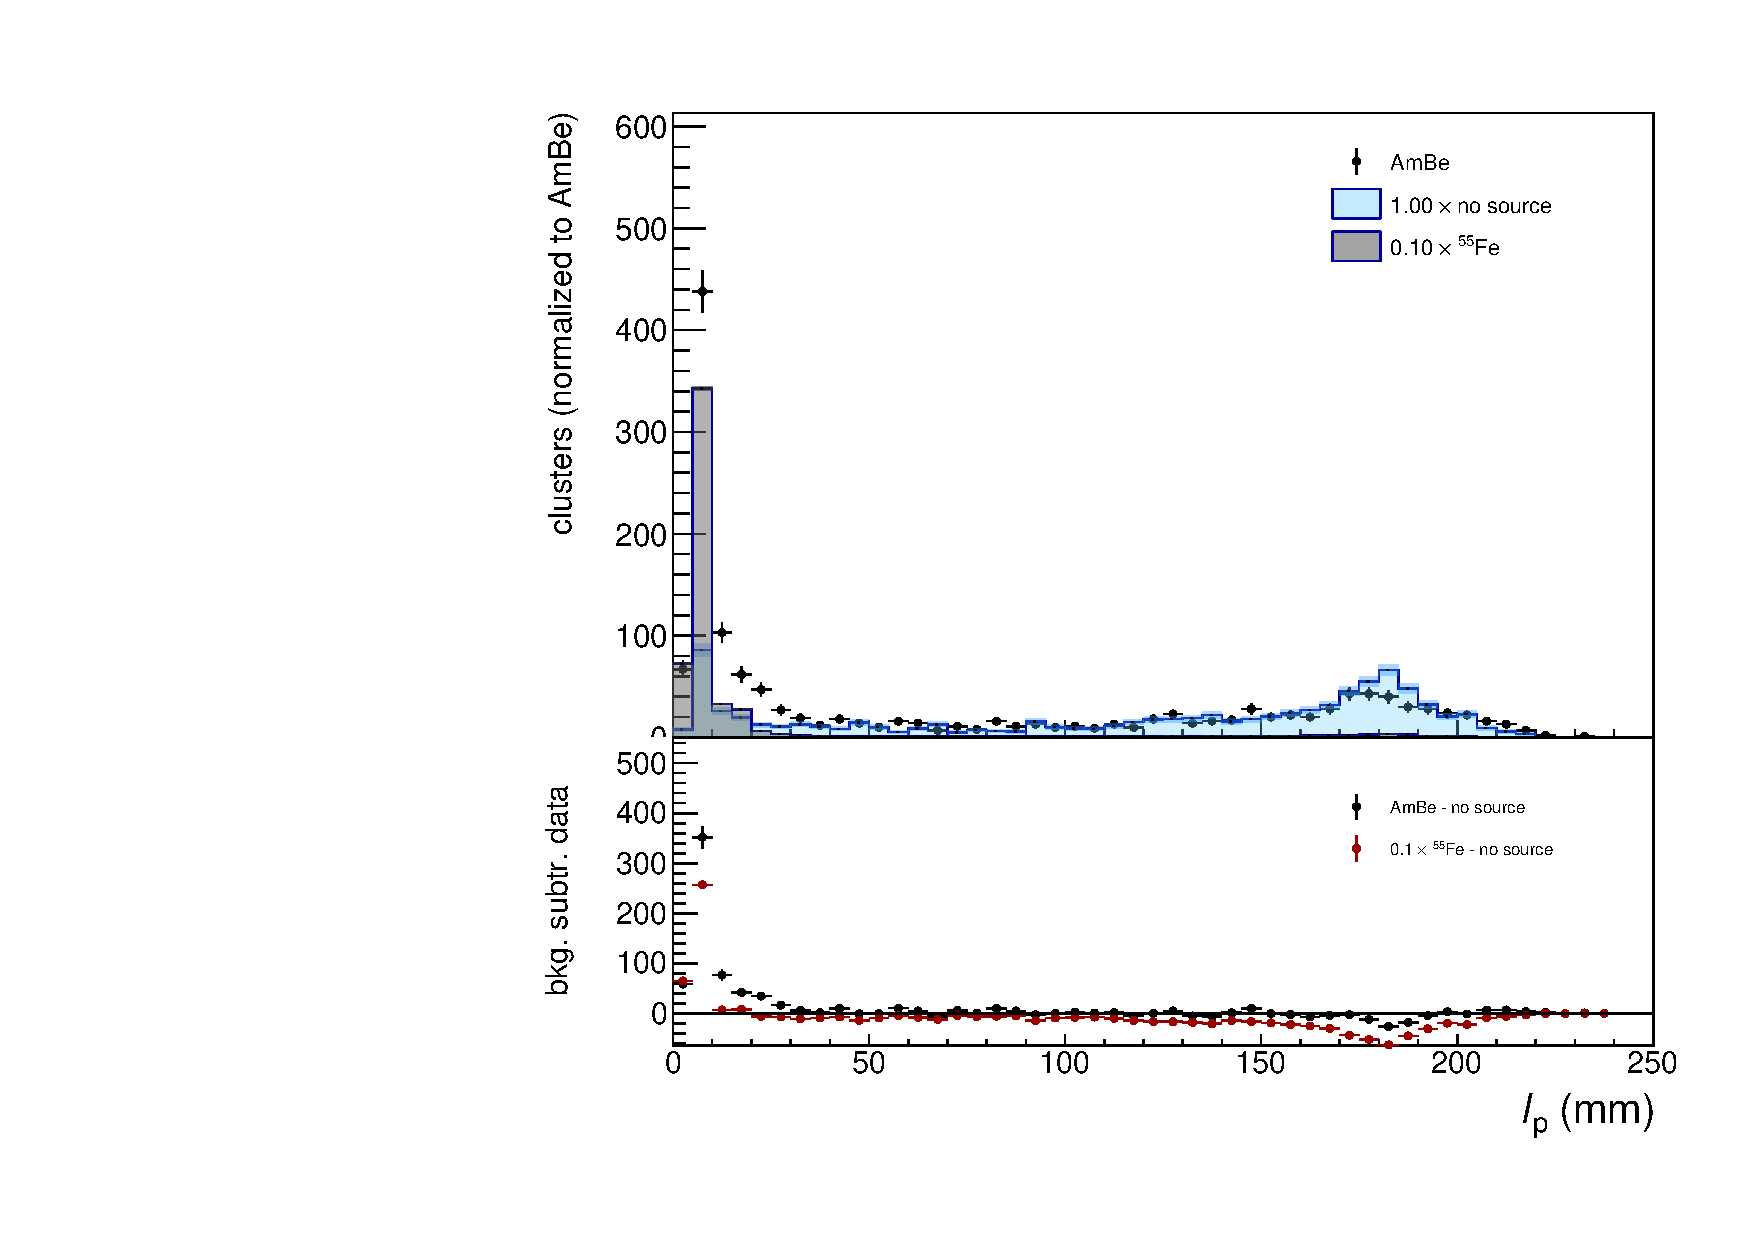
\includegraphics[width=0.45\linewidth]{figures/length}
  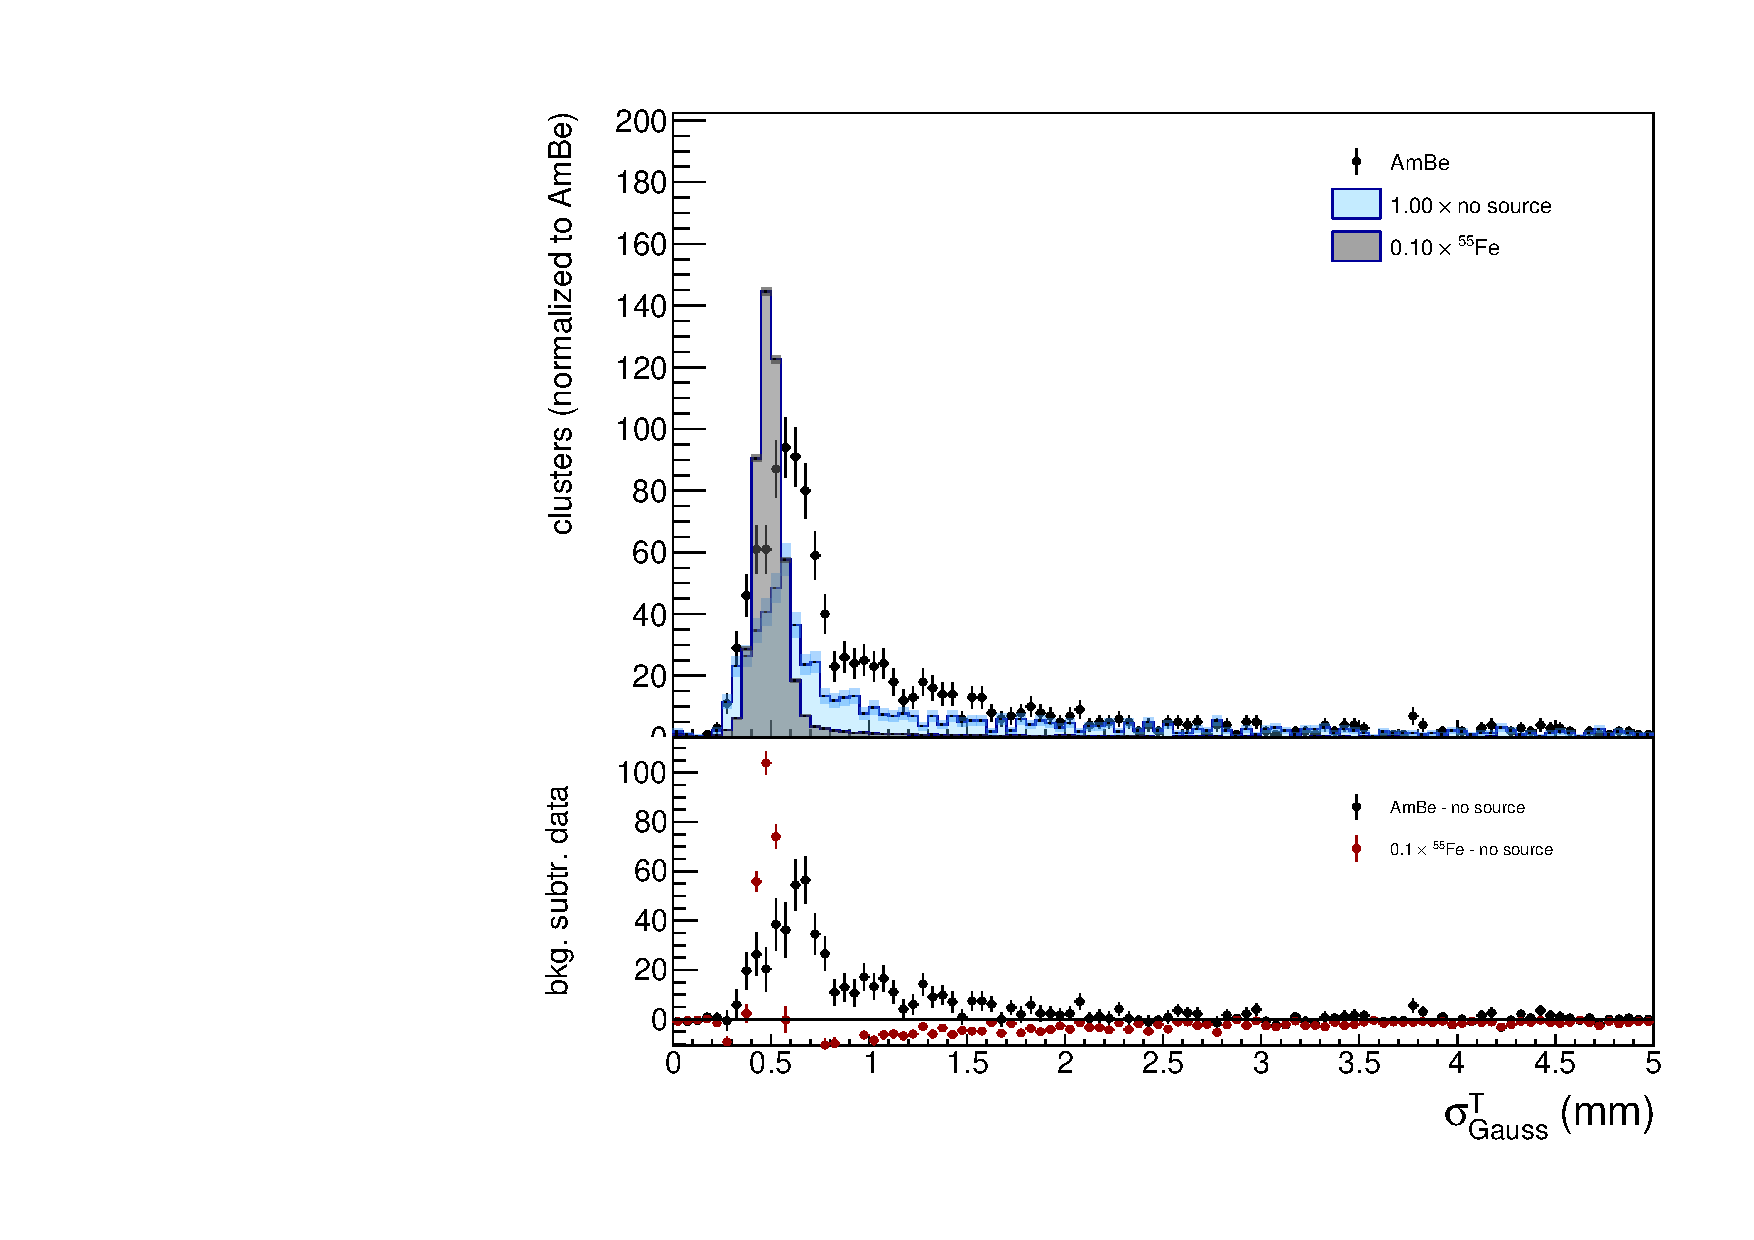
\includegraphics[width=0.45\linewidth]{figures/tgausssigma}

  \caption{Supercluster sizes projected onto the $x$--$y$ plane. Left:
    longitudinal path length, $l_p$.  Right: transverse Gaussian
    spread, \tsigmag. Filled points represent data with \ambe source,
    dark gray (light blue) distribution represents data with \fe
    source (no source).  The normalization of data without any artificial source is scaled
    to the same exposure time of the \ambe one. For the data with \fe source ,
    a scaling factor of one tenth is applied for clearness, given the
    larger activity of this source.  \label{fig:clsize}}

    \end{center}
\end{figure}

As described in Sec.~\ref{sec:layout}, each pixel images an area of
$125\times125$\unit{$\mu$m$^2$}. Thus the cluster sizes distributions
show an average Gaussian width for the \fe spots
$\tsigmag\approx500$\unit{$\mu$m} (dominated by the diffusion in the
gas), while it is larger, approximately 625\unit{$\mu$m}, for data
with \ambe source.  The contribution of cosmic rays, present in all
the data, is clearly visible in the data without any artificial radioactive
source, corresponding to clusters with a length similar to the detector transverse
size (22\unit{cm}).

Other observables  are the slimness,
$\xi$, and the light density, $\delta$, shown in
Fig.~\ref{fig:clshape}. The former is a useful handle to reject tracks
from cosmic rays, which  typically have  a slim aspect ratio, \ie, low
values of $\xi$, while the clusters from \fe are almost round, with
values of $\xi\approx 1$. Data with \ambe source, which contains  a
component of nuclear recoils, show a component of round spots,
similar in size to the ones of \fe, and a more elliptical component,
with $0.4<\xi<0.8$ values. Finally, the light density, $\delta$, is the
variable expected to better discriminate among different
candidates: cosmic rays induced background, electron recoils and
nuclear recoil candidates. This is the variable used for the final
particle identification.

\begin{figure}[ht]
  \begin{center}
  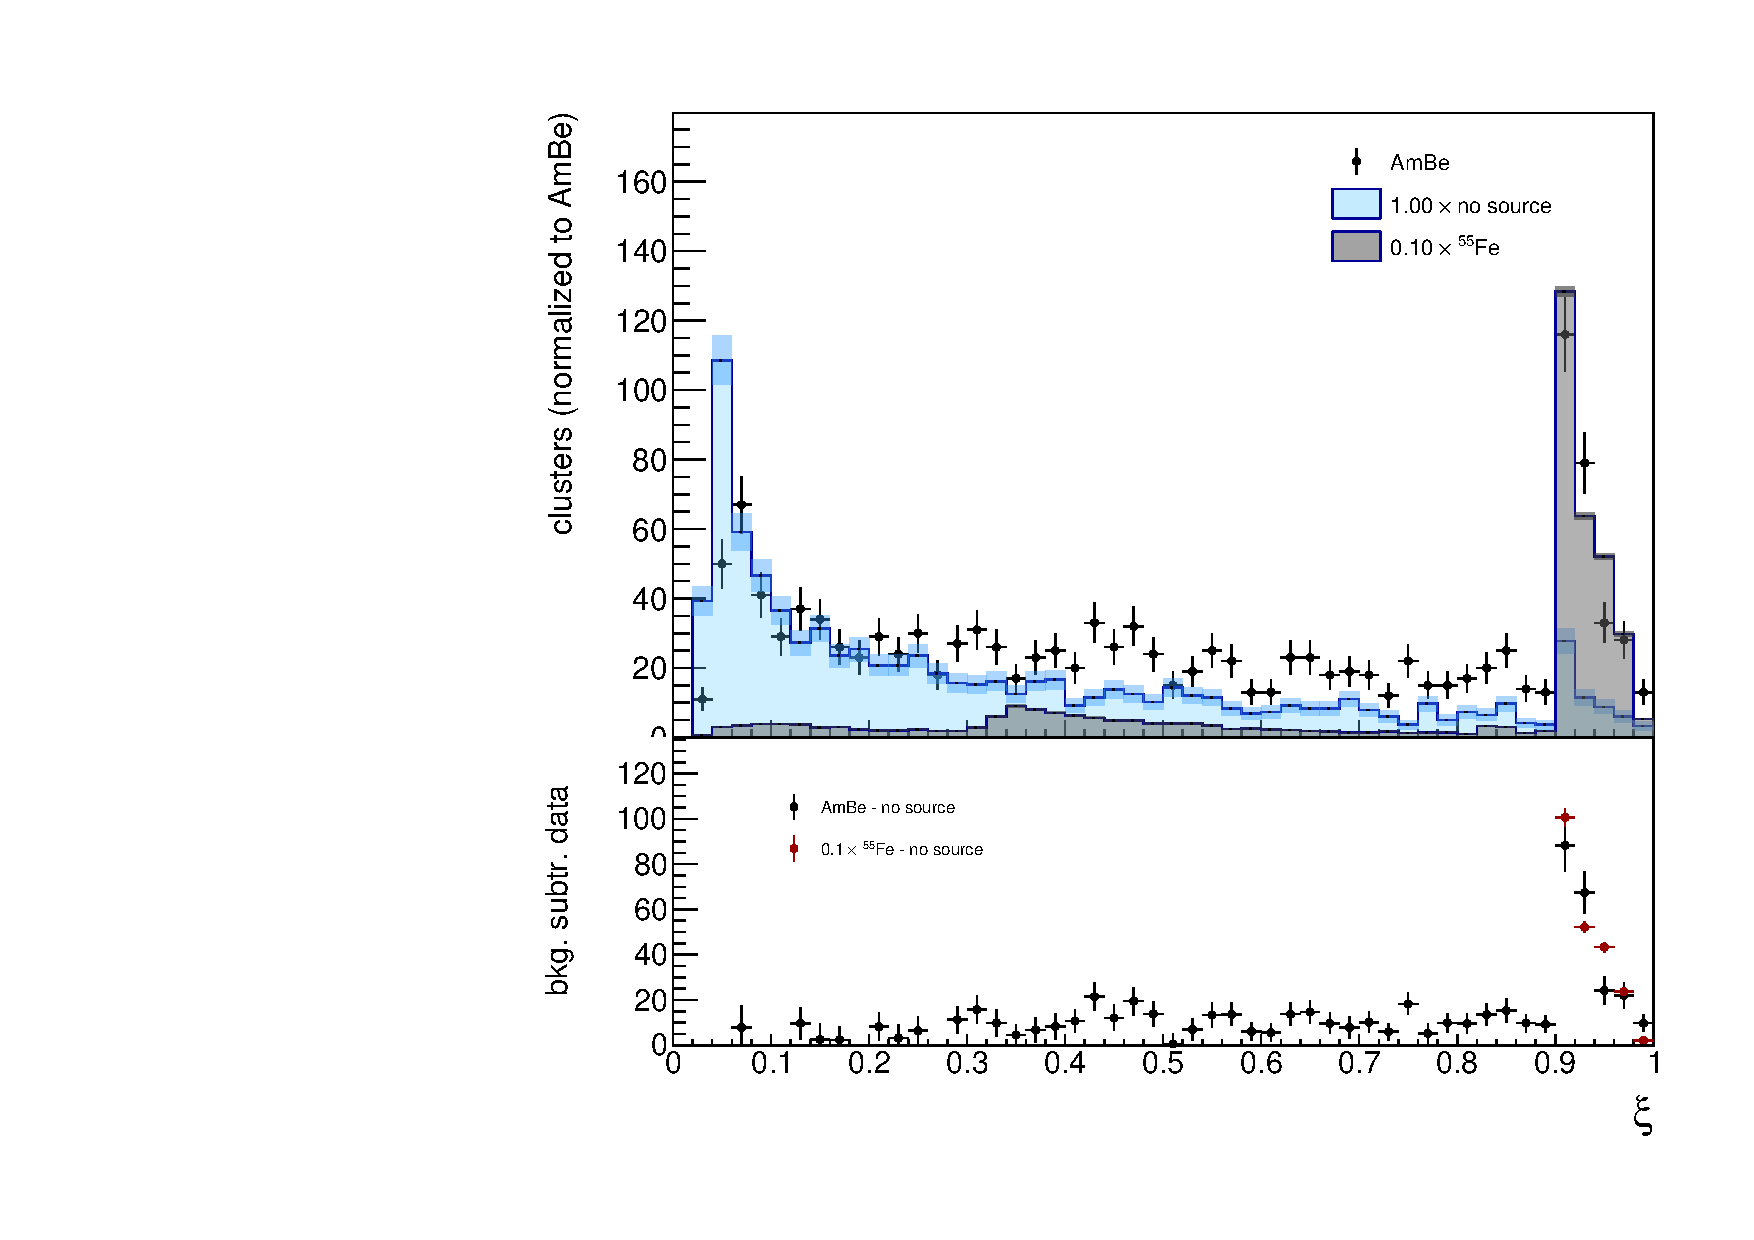
\includegraphics[width=0.45\linewidth]{figures/slimness}
  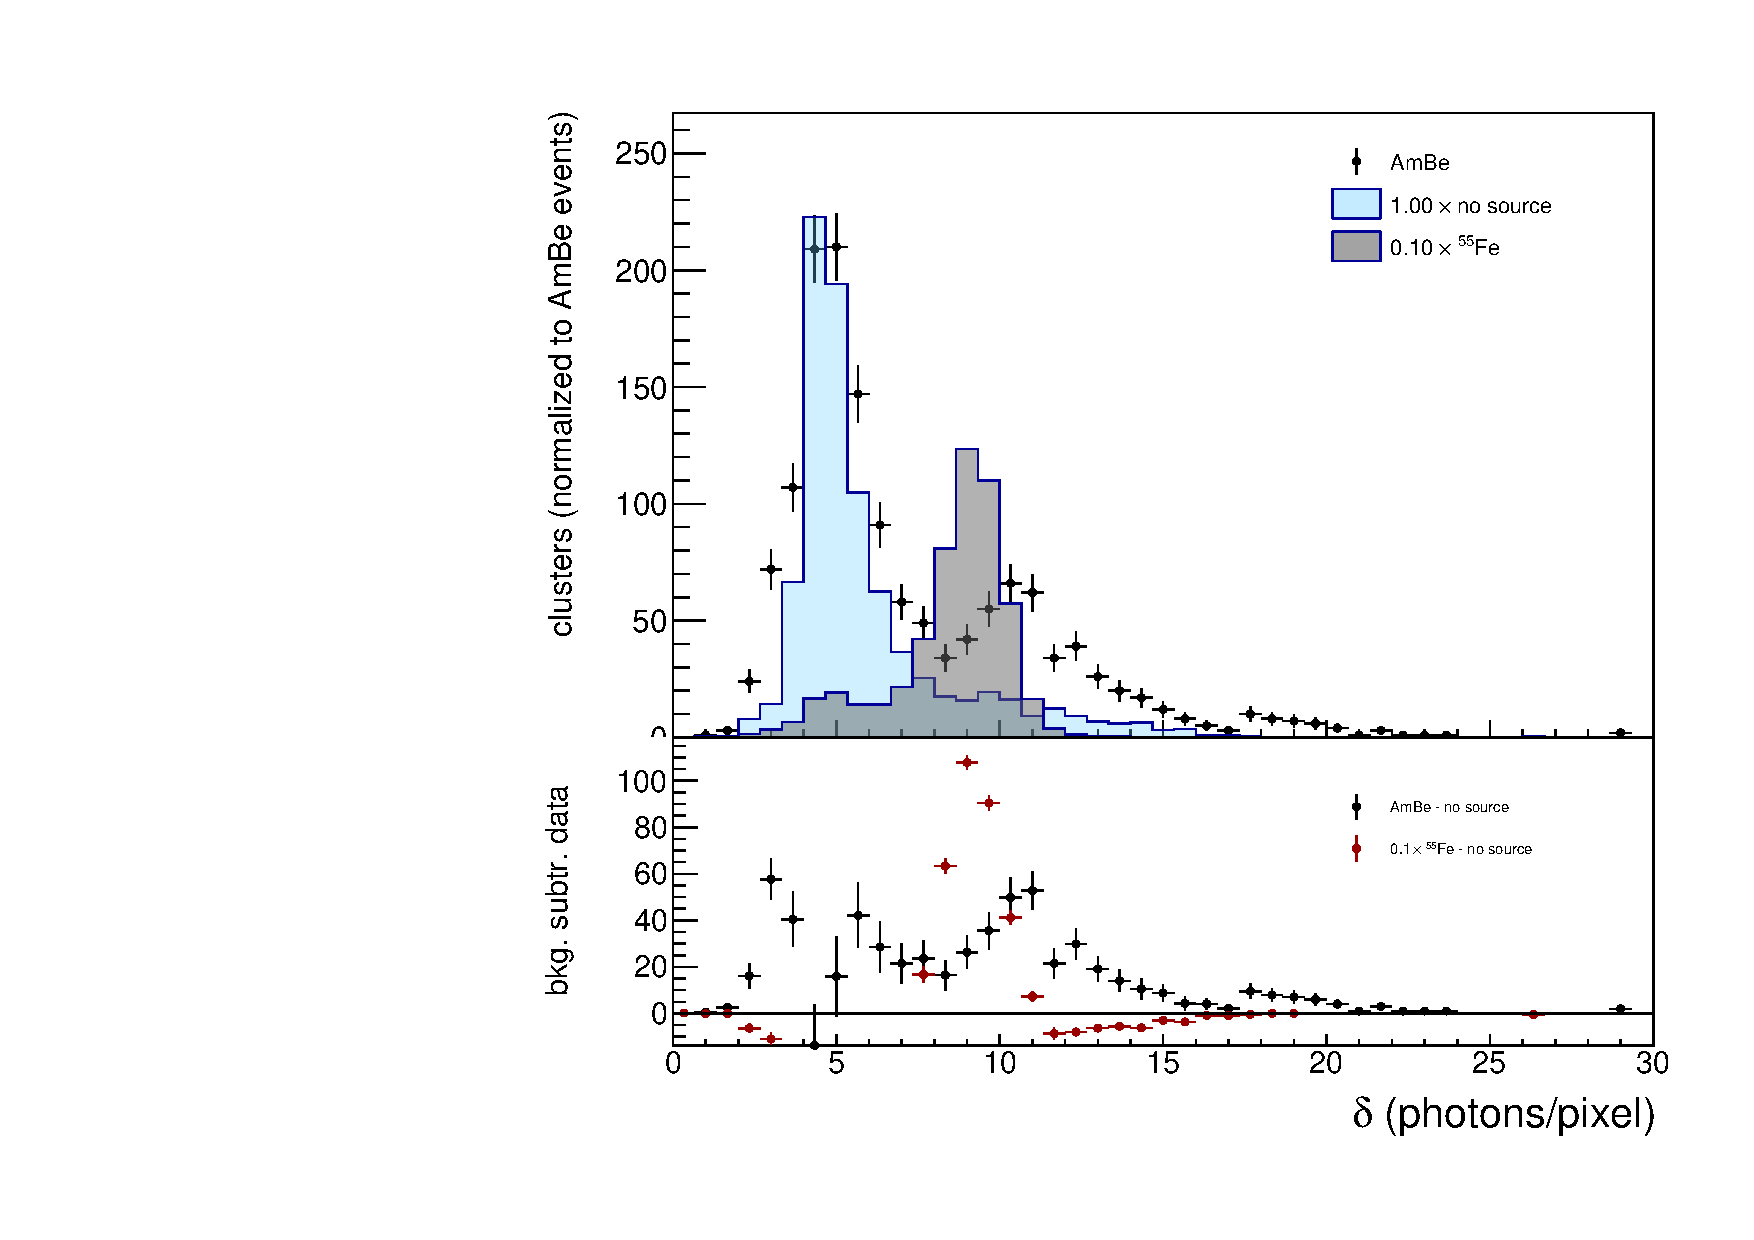
\includegraphics[width=0.45\linewidth]{figures/density}

  \caption{Supercluster variables. Left: slimness $\xi$; right: light
    density $\delta$. Filled points represent data with \ambe source,
    dark gray (light blue) distribution represents data with \fe
    source (no source).  The normalization of data without source is
    to the same exposure time of the \ambe one. For the data with \fe,
    a scaling factor of one tenth is applied for clearness, given the
    larger activity of this source. \label{fig:clshape}}

\end{center}
\end{figure}

Finally, Fig.~\ref{fig:energy} shows the calibrated energy ($E$)
spectrum for the reconstructed superclusters and the average projected
\dedl. The energy spectrum shows the $E=5.9\keV$ for data
with \fe source, and a characteristic broad peak for cosmic rays
tracks at around 60\keV. The distribution of the observed
\dedl for the no-source sample and for the \ambe
samples. The broadening of the distribution is mainly due to the
specific energy loss fluctuation in the gas mixture of the cosmic ray
particles.  Its modal value, corrected for the effect of the angular
distribution (an average inclination of 56$^{\circ}$ was measured from
track reconstruction) is 2.5~\keV/cm, in good agreement with
the \garfield prediction of 2.3~\keV/cm.

\begin{figure}[ht]
  \begin{center}
  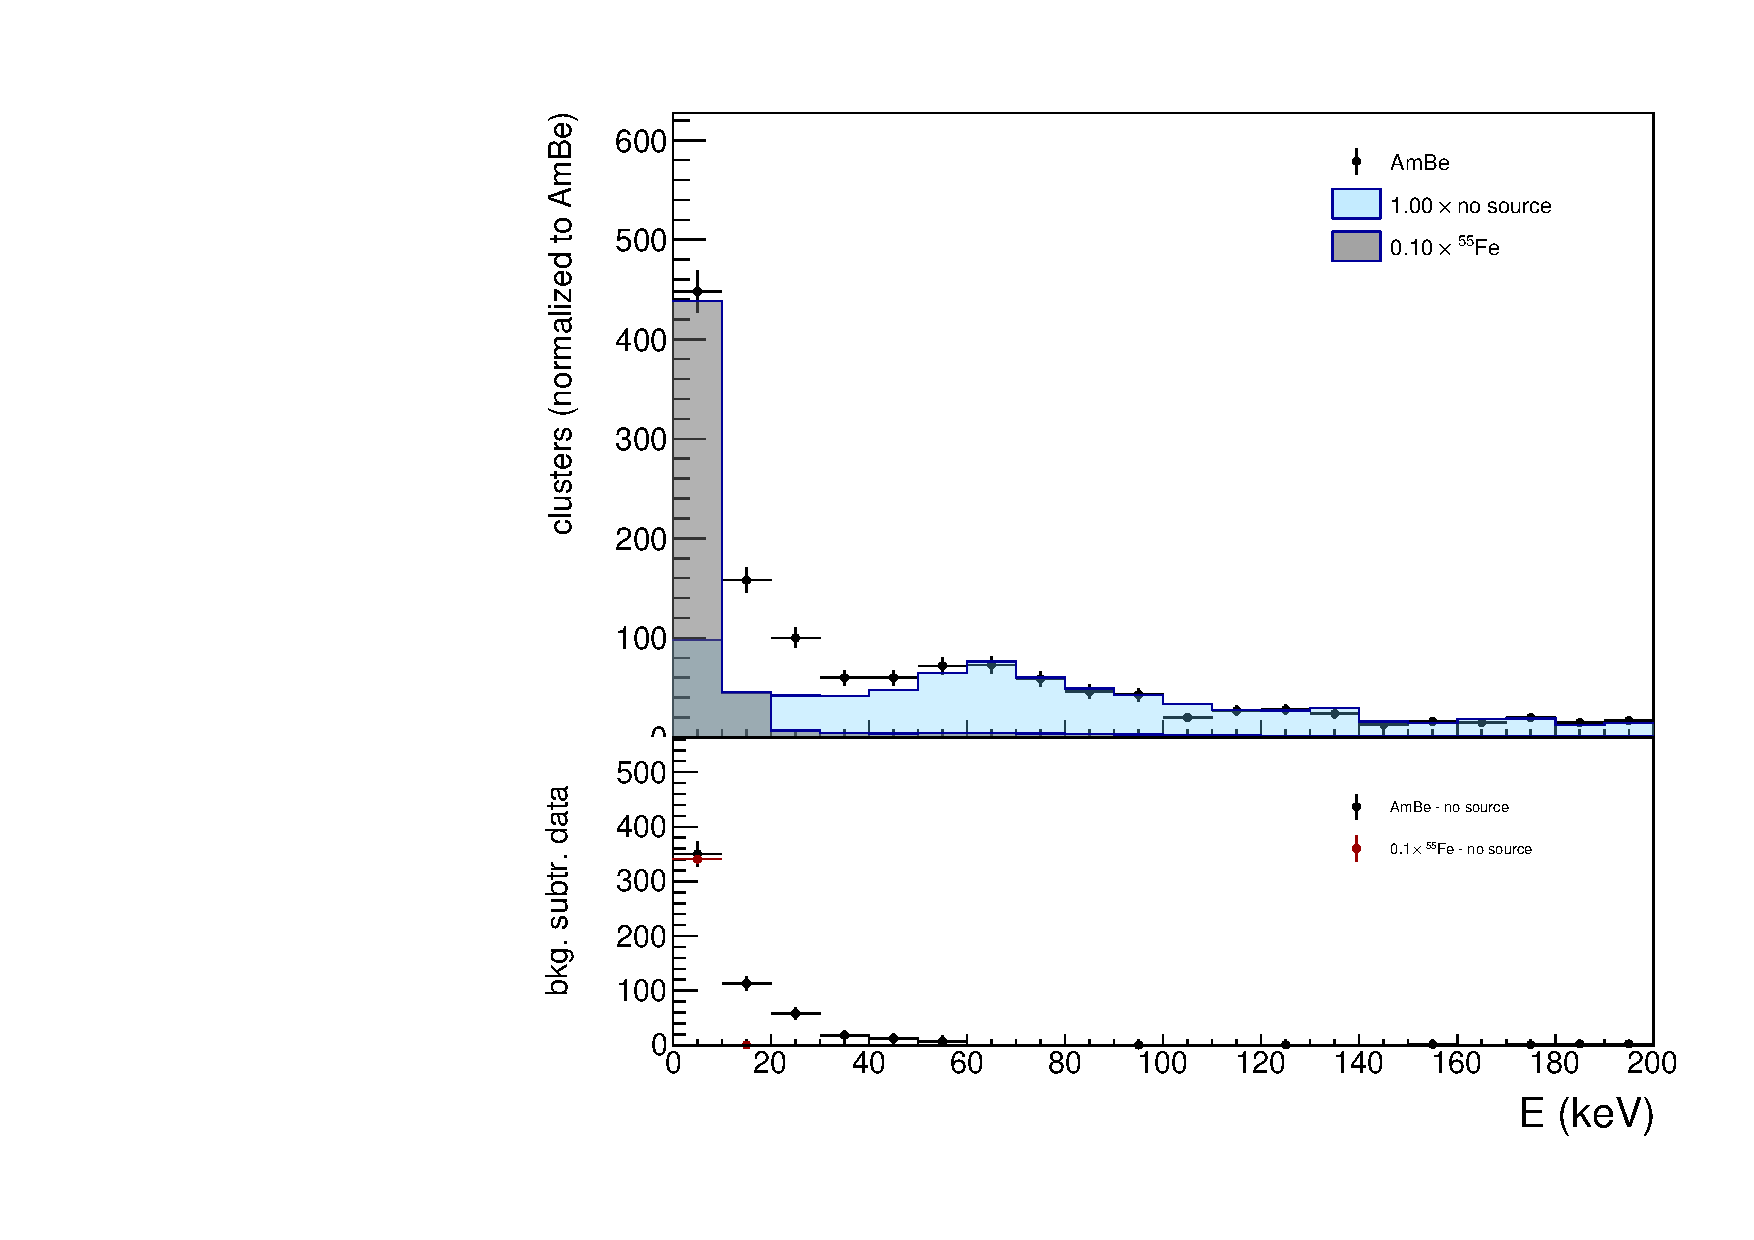
\includegraphics[width=0.45\linewidth]{figures/energyExt}
  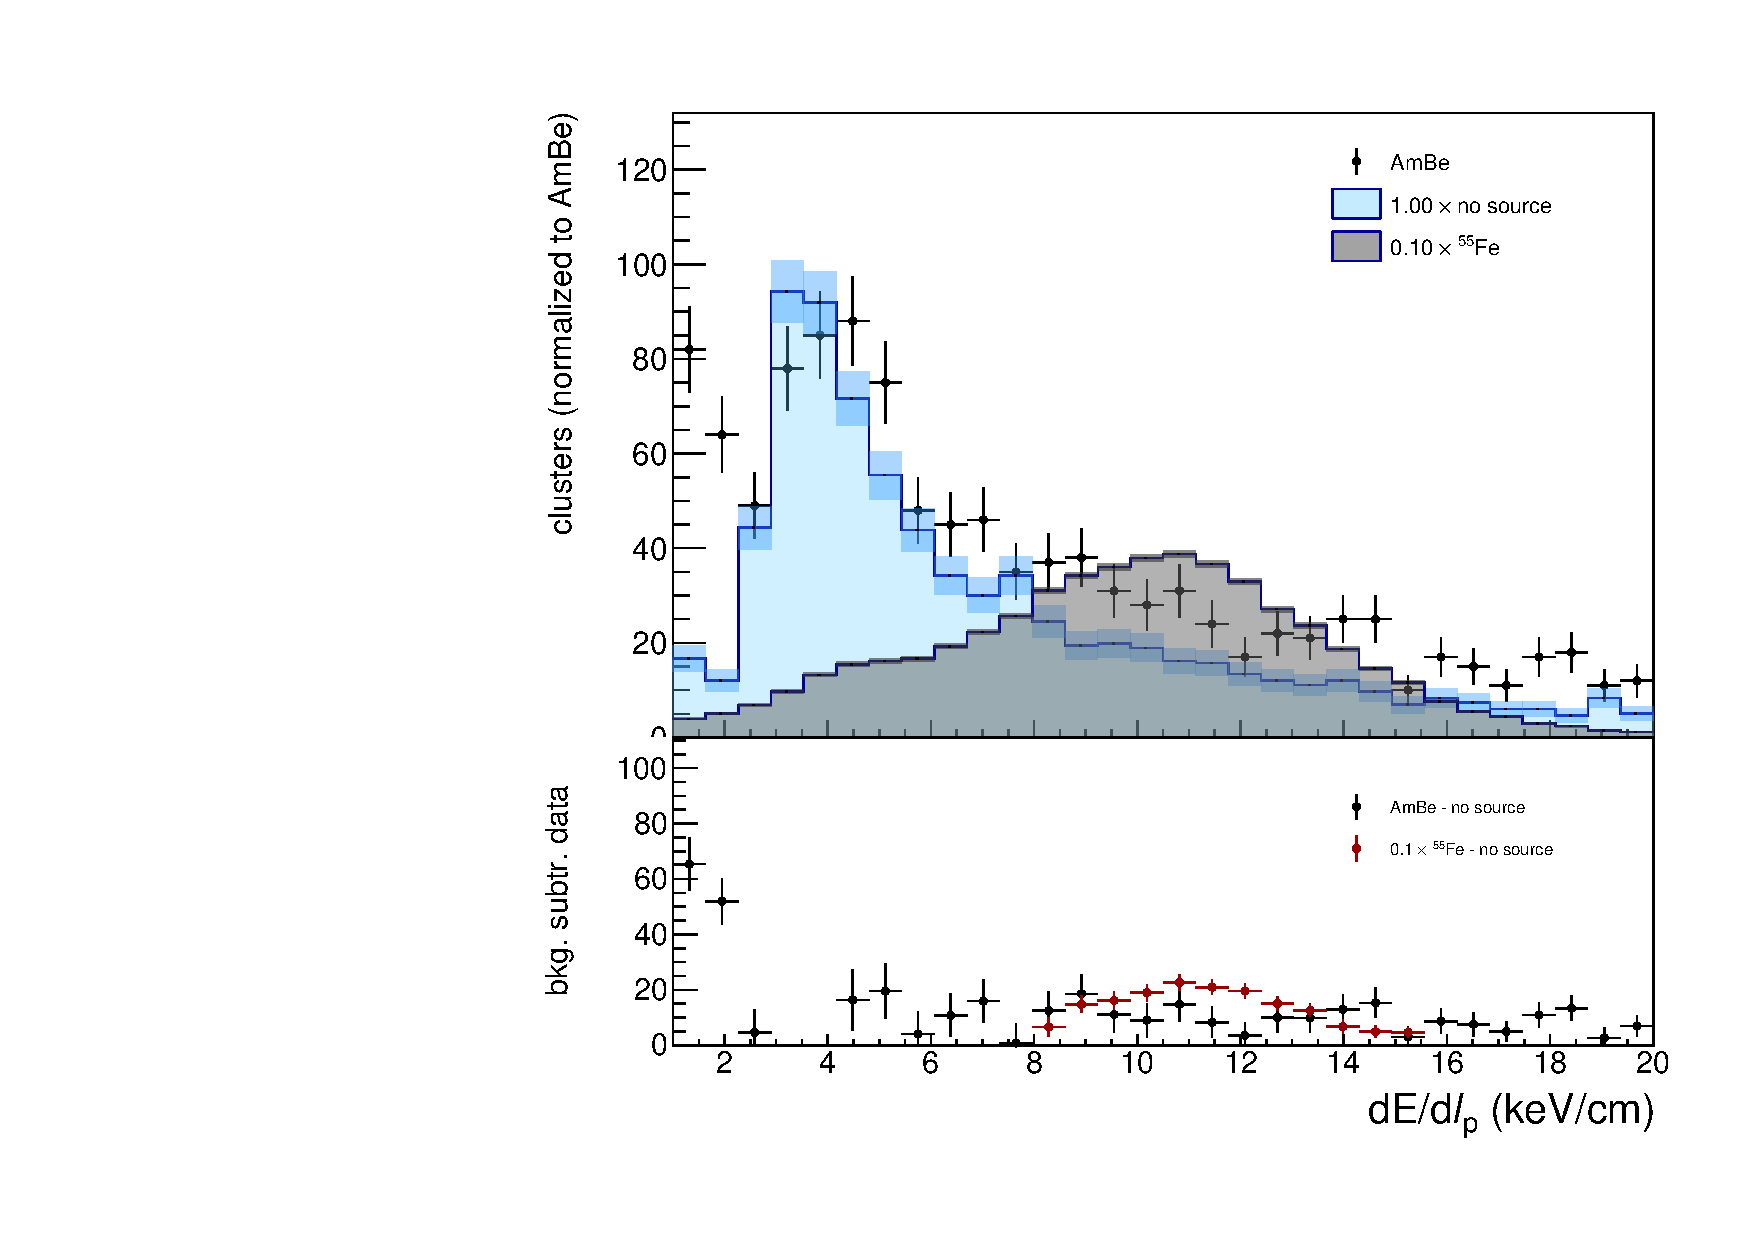
\includegraphics[width=0.45\linewidth]{figures/dedx}

  \caption{Supercluster calibrated energy spectrum (left) and their
    average \dedl. Filled points represent data with \ambe source,
    dark gray (light blue) distribution represents data with \fe
    source (no source).  The normalization of data without source is
    to the same exposure time of the \ambe one. For the data with \fe,
    a scaling factor of one tenth is applied for clearness, given the
    larger activity of this source. \label{fig:energy}}

\end{center}
\end{figure}

\subsection{Background normalization}
\label{sec:background}
The data with \ambe source, taken on the Earth surface, suffers from a
large contribution of interactions of cosmic rays. The cluster shape
observables provide a powerful handle to discriminate them from nuclear
recoils candidates, but the small residual background needs to be
statistically subtracted. The distributions shown earlier, where the
different types of data are normalized to the same exposure time,
demonstrate that the live-time normalization provides already a good
estimate of the amount of  cosmic rays  in data with artificial
radioactive sources. This approach does not account for a possible bias
from the trigger, which is generated by the PMT signals, as described
in Sec.~\ref{sec:layout}. Indeed, in runs with the \ambe source, the
PMT can trigger both on signals from neutron recoils or photons
produced by the $^{241}$Am, and on ubiquitous signals from cosmic
rays, while in the sample without source only the latter is possible.
This implies that, during the same exposure time, the probability to
trigger on cosmic rays is lower in events with \ambe than in no-source events. The trigger efficiency scale factor,
$\varepsilon_{SF}$, can be obtained as the ratio of the number of
clusters selected in pure control samples of cosmic rays ($CR$)
obtained on both types of runs:
\begin{equation}
\label{eq:sfeff}
\varepsilon_{SF} = \frac{N^{AmBe}_{CR}}{N^{no-source}_{CR}}.
\end{equation}

The $CR$ control region is defined by selecting clusters with
$l>13$\unit{cm}, $\xi<0.1$, $\tsigmag<6$\unit{mm}, having an energy
within a range dominated by the cosmic rays contribution,
$50<E<80\keV$. The selected clusters show small values of
$\delta\approx5$, well compatible with the small specific ionization
of ultra-relativistic particles.  This sample is limited in
statistics, but it is expected to be almost 100\% pure. The scale
factor obtained is $\varepsilon_{SF}=0.75\pm0.02$.

In Fig.~\ref{fig:cosmics} the typical light density and polar angle
(with respect the horizontal axis) distributions for long clusters of
any energy, still dominated by cosmic rays, are shown for the \ambe
and for the no-source sample, after having applied the
$\varepsilon_{SF}$ scale factor to the latter. Clusters with
$\delta<6$ are thus expected to be mostly coming from cosmic tracks,
and they show indeed a polar angle which is shifted at values towards
$90^\circ$.


\begin{figure}[ht]
  \begin{center}
  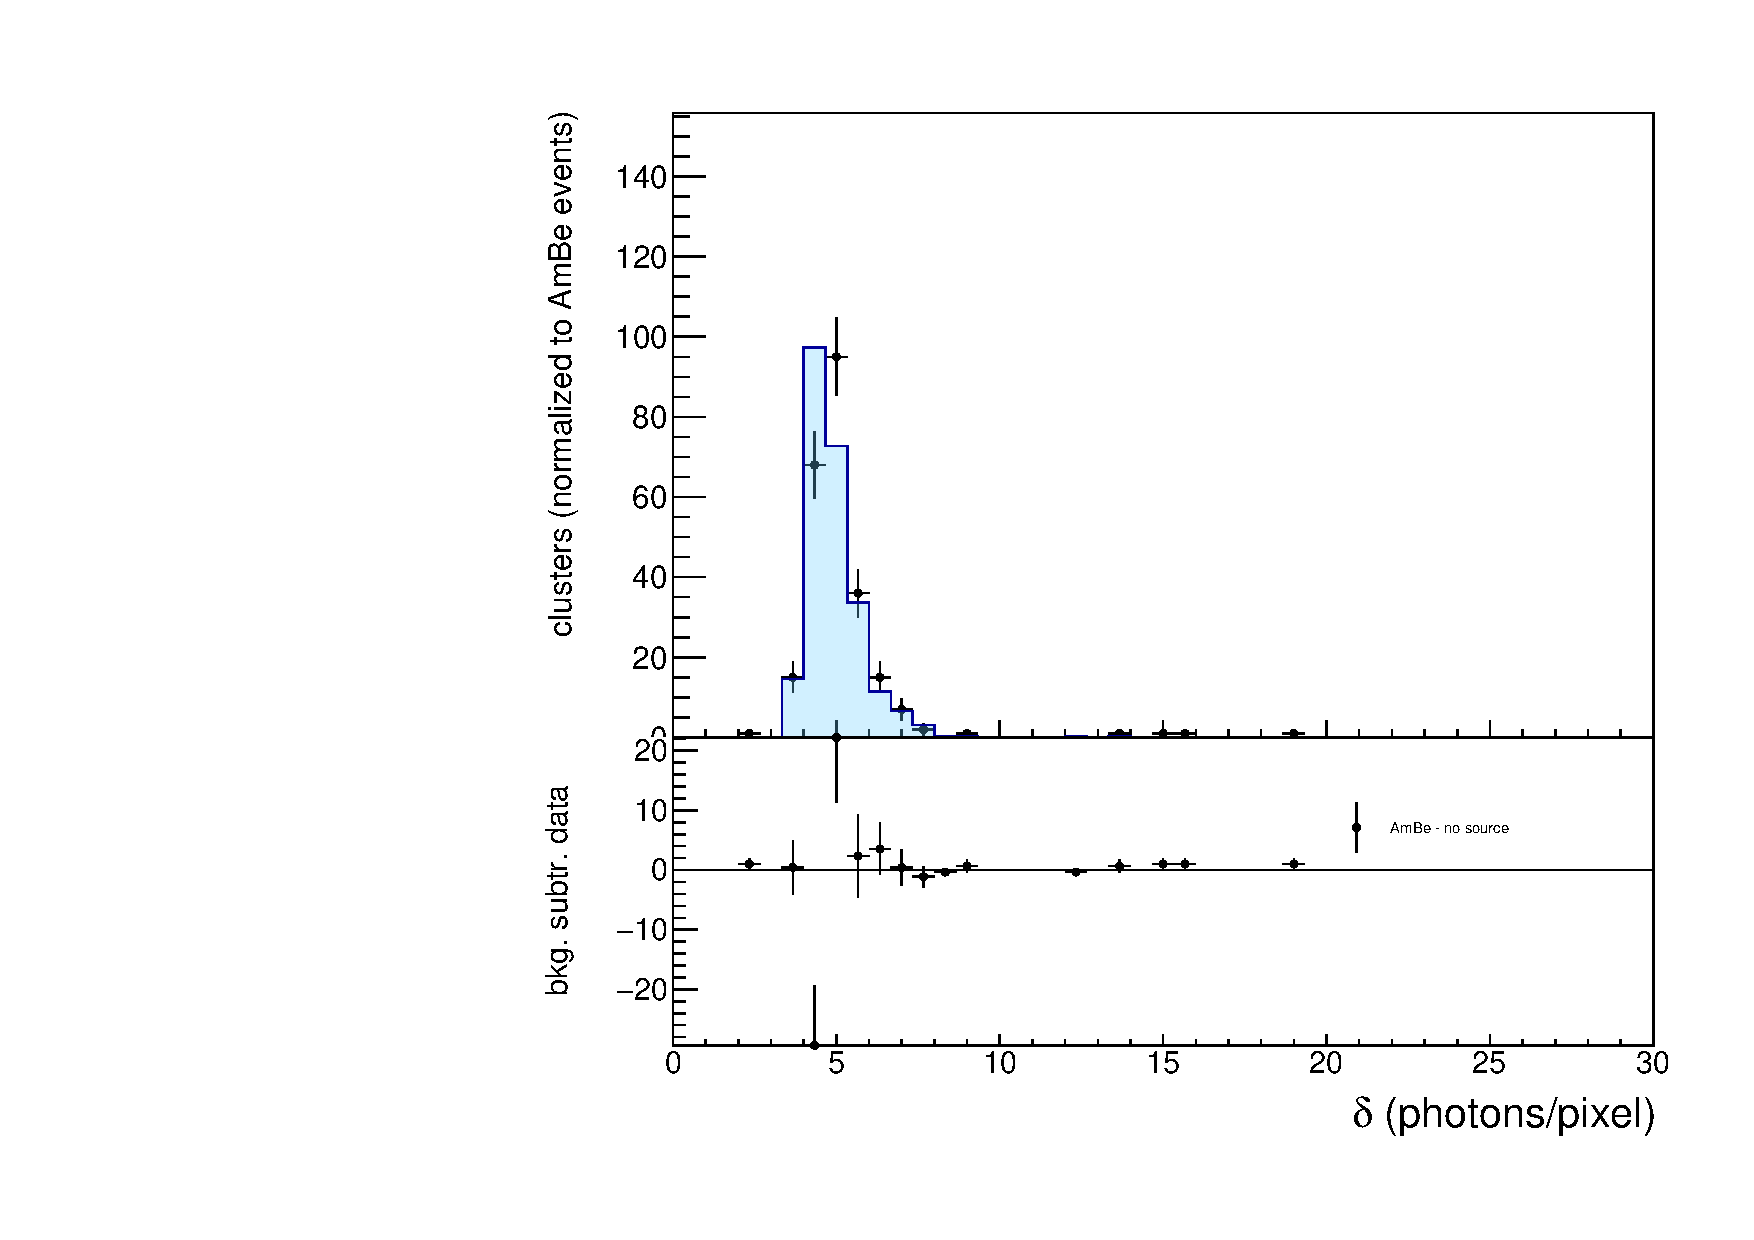
\includegraphics[width=0.45\linewidth]{figures/density_cosmics}
  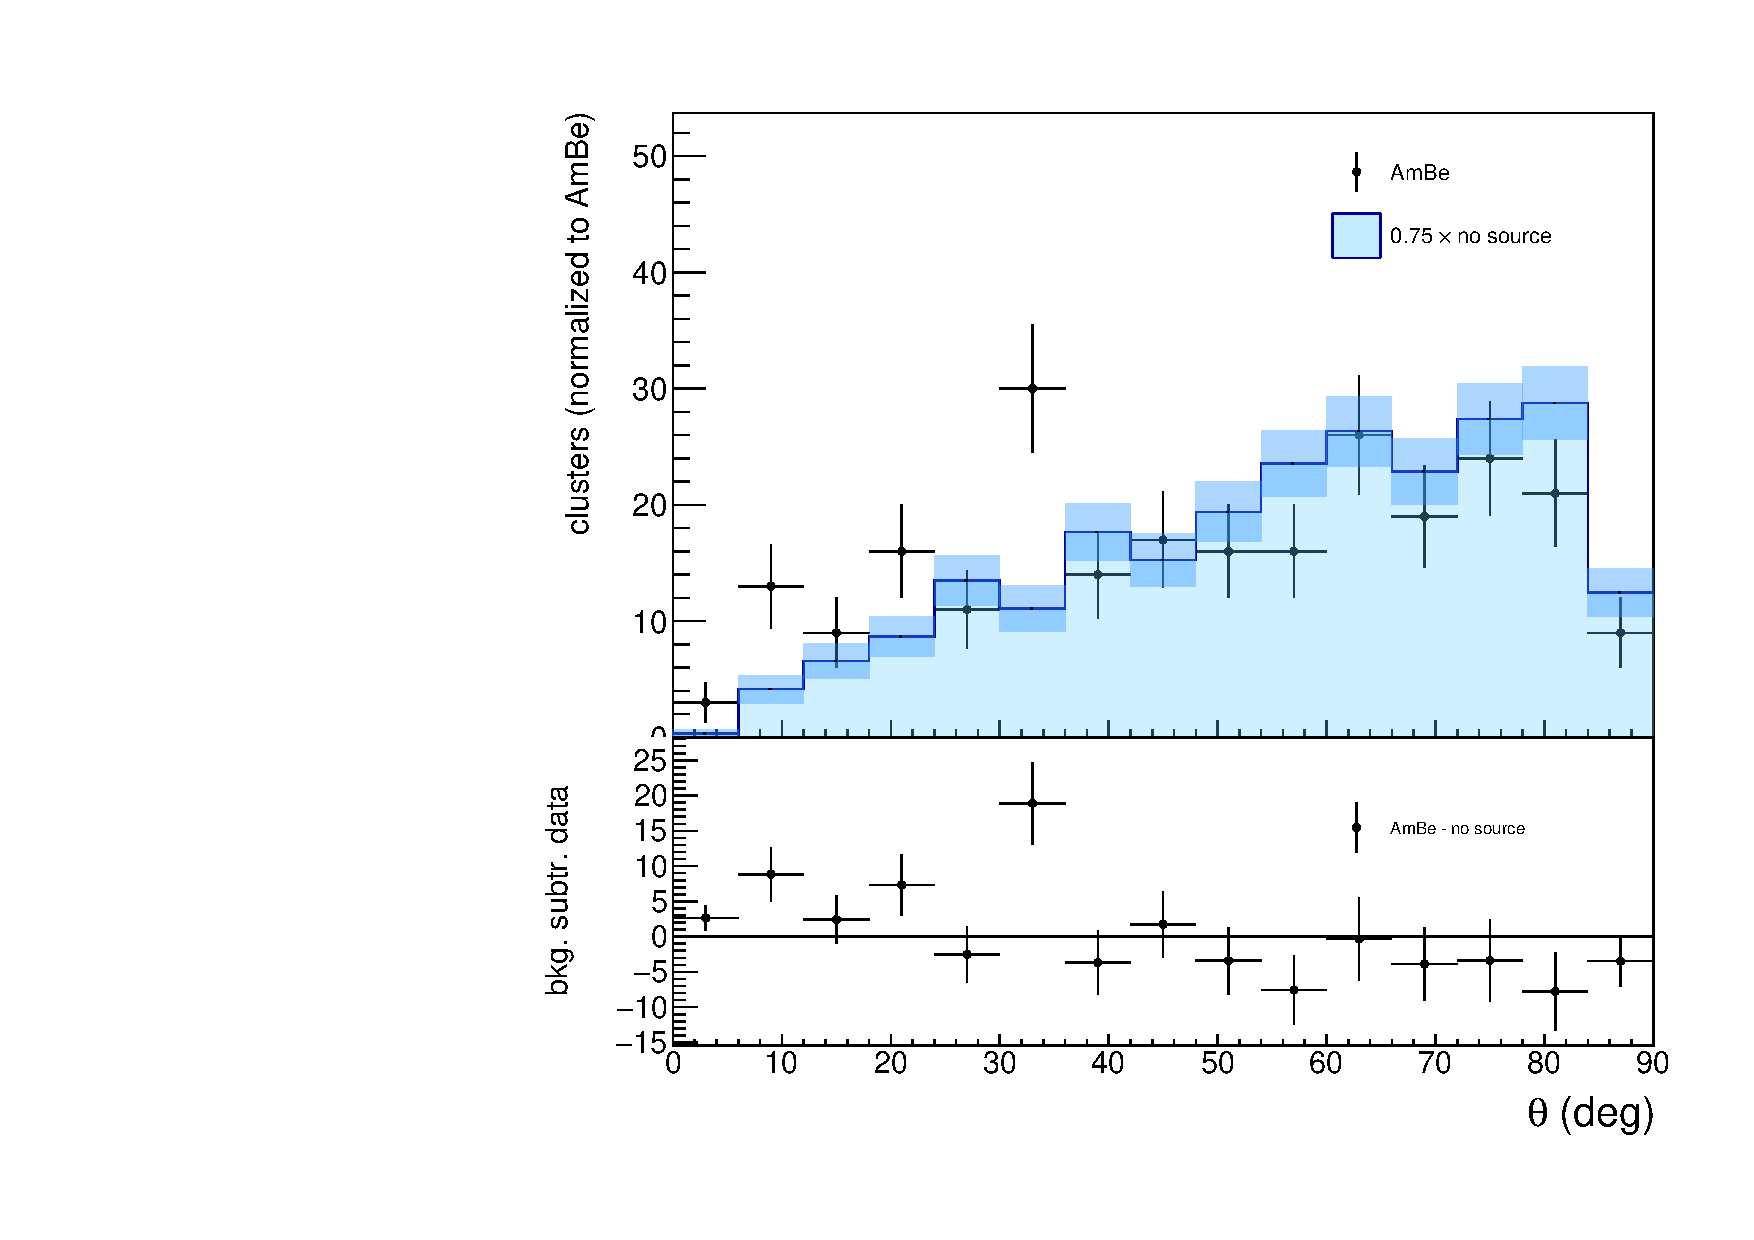
\includegraphics[width=0.45\linewidth]{figures/inclination_cosmics}

  \caption{Supercluster light density $\delta$ (left) and  polar
    angle (right) -   with respect the horizontal axis - distributions  for long clusters,
    dominated by cosmic rays tracks.  Filled points represent data
    with \ambe source, light blue distribution represents data without
    any artificial source.  The normalization of data without source is to the
    same exposure time of the \ambe one, accounting for the trigger
    scale factor $\varepsilon_{SF}$, as defined in the
    text.  \label{fig:cosmics}}

\end{center}
\end{figure}
